\documentclass[1p]{elsarticle_modified}
%\bibliographystyle{elsarticle-num}

%\usepackage[colorlinks]{hyperref}
%\usepackage{abbrmath_seonhwa} %\Abb, \Ascr, \Acal ,\Abf, \Afrak
\usepackage{amsfonts}
\usepackage{amssymb}
\usepackage{amsmath}
\usepackage{amsthm}
\usepackage{scalefnt}
\usepackage{amsbsy}
\usepackage{kotex}
\usepackage{caption}
\usepackage{subfig}
\usepackage{color}
\usepackage{graphicx}
\usepackage{xcolor} %% white, black, red, green, blue, cyan, magenta, yellow
\usepackage{float}
\usepackage{setspace}
\usepackage{hyperref}

\usepackage{tikz}
\usetikzlibrary{arrows}

\usepackage{multirow}
\usepackage{array} % fixed length table
\usepackage{hhline}

%%%%%%%%%%%%%%%%%%%%%
\makeatletter
\renewcommand*\env@matrix[1][\arraystretch]{%
	\edef\arraystretch{#1}%
	\hskip -\arraycolsep
	\let\@ifnextchar\new@ifnextchar
	\array{*\c@MaxMatrixCols c}}
\makeatother %https://tex.stackexchange.com/questions/14071/how-can-i-increase-the-line-spacing-in-a-matrix
%%%%%%%%%%%%%%%

\usepackage[normalem]{ulem}

\newcommand{\msout}[1]{\ifmmode\text{\sout{\ensuremath{#1}}}\else\sout{#1}\fi}
%SOURCE: \msout is \stkout macro in https://tex.stackexchange.com/questions/20609/strikeout-in-math-mode

\newcommand{\cancel}[1]{
	\ifmmode
	{\color{red}\msout{#1}}
	\else
	{\color{red}\sout{#1}}
	\fi
}

\newcommand{\add}[1]{
	{\color{blue}\uwave{#1}}
}

\newcommand{\replace}[2]{
	\ifmmode
	{\color{red}\msout{#1}}{\color{blue}\uwave{#2}}
	\else
	{\color{red}\sout{#1}}{\color{blue}\uwave{#2}}
	\fi
}

\newcommand{\Sol}{\mathcal{S}} %segment
\newcommand{\D}{D} %diagram
\newcommand{\A}{\mathcal{A}} %arc


%%%%%%%%%%%%%%%%%%%%%%%%%%%%%5 test

\def\sl{\operatorname{\textup{SL}}(2,\Cbb)}
\def\psl{\operatorname{\textup{PSL}}(2,\Cbb)}
\def\quan{\mkern 1mu \triangleright \mkern 1mu}

\theoremstyle{definition}
\newtheorem{thm}{Theorem}[section]
\newtheorem{prop}[thm]{Proposition}
\newtheorem{lem}[thm]{Lemma}
\newtheorem{ques}[thm]{Question}
\newtheorem{cor}[thm]{Corollary}
\newtheorem{defn}[thm]{Definition}
\newtheorem{exam}[thm]{Example}
\newtheorem{rmk}[thm]{Remark}
\newtheorem{alg}[thm]{Algorithm}

\newcommand{\I}{\sqrt{-1}}
\begin{document}

%\begin{frontmatter}
%
%\title{Boundary parabolic representations of knots up to 8 crossings}
%
%%% Group authors per affiliation:
%\author{Yunhi Cho} 
%\address{Department of Mathematics, University of Seoul, Seoul, Korea}
%\ead{yhcho@uos.ac.kr}
%
%
%\author{Seonhwa Kim} %\fnref{s_kim}}
%\address{Center for Geometry and Physics, Institute for Basic Science, Pohang, 37673, Korea}
%\ead{ryeona17@ibs.re.kr}
%
%\author{Hyuk Kim}
%\address{Department of Mathematical Sciences, Seoul National University, Seoul 08826, Korea}
%\ead{hyukkim@snu.ac.kr}
%
%\author{Seokbeom Yoon}
%\address{Department of Mathematical Sciences, Seoul National University, Seoul, 08826,  Korea}
%\ead{sbyoon15@snu.ac.kr}
%
%\begin{abstract}
%We find all boundary parabolic representation of knots up to 8 crossings.
%
%\end{abstract}
%\begin{keyword}
%    \MSC[2010] 57M25 
%\end{keyword}
%
%\end{frontmatter}

%\linenumbers
%\tableofcontents
%
\newcommand\colored[1]{\textcolor{white}{\rule[-0.35ex]{0.8em}{1.4ex}}\kern-0.8em\color{red} #1}%
%\newcommand\colored[1]{\textcolor{white}{ #1}\kern-2.17ex	\textcolor{white}{ #1}\kern-1.81ex	\textcolor{white}{ #1}\kern-2.15ex\color{red}#1	}

{\Large $\underline{12n_{0351}~(K12n_{0351})}$}

\setlength{\tabcolsep}{10pt}
\renewcommand{\arraystretch}{1.6}
\vspace{1cm}\begin{tabular}{m{100pt}>{\centering\arraybackslash}m{274pt}}
\multirow{5}{120pt}{
	\centering
	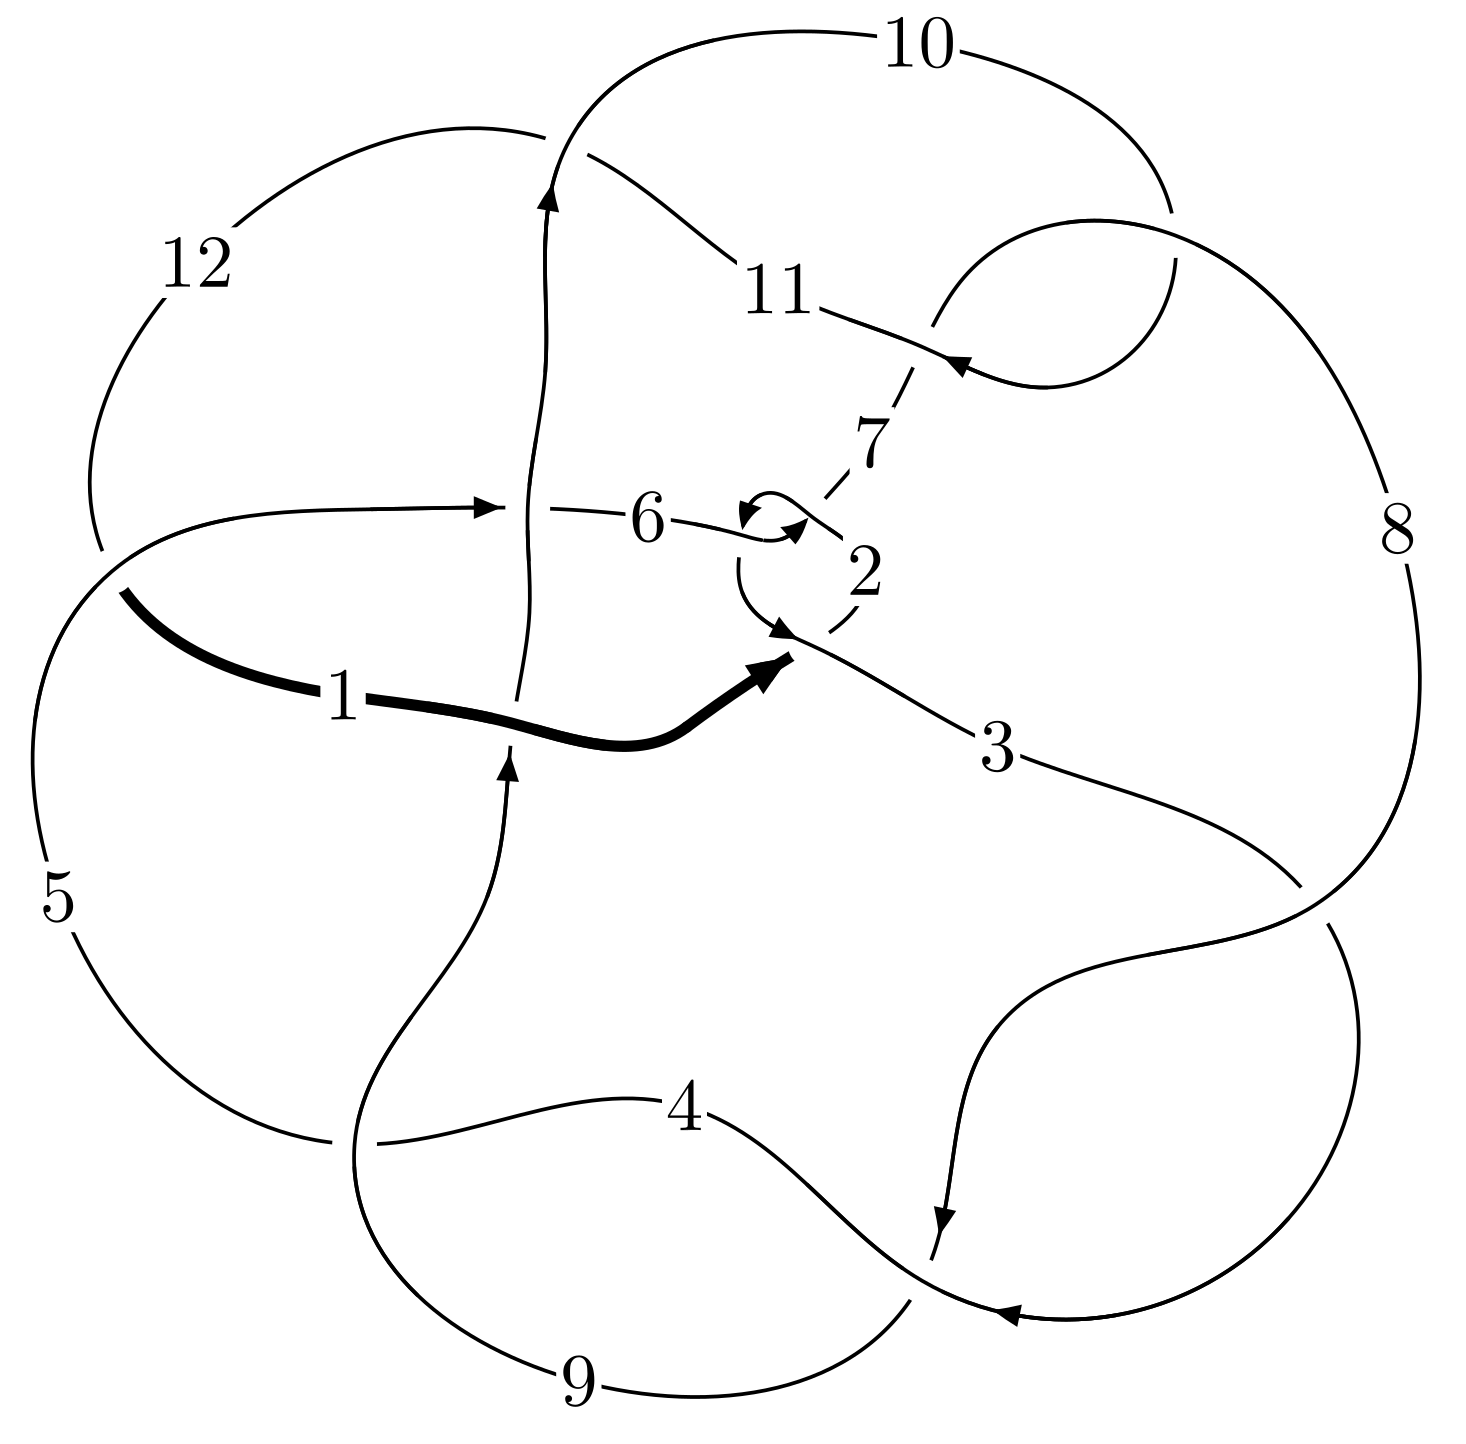
\includegraphics[width=112pt]{../../../GIT/diagram.site/Diagrams/png/2440_12n_0351.png}\\
\ \ \ A knot diagram\footnotemark}&
\allowdisplaybreaks
\textbf{Linearized knot diagam} \\
\cline{2-2}
 &
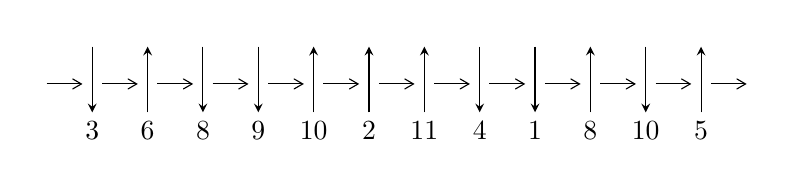
\begin{tikzpicture}[x=20pt, y=17pt]
	% nodes
	\node (C0) at (0, 0) {};
	\node (C1) at (1, 0) {};
	\node (C1U) at (1, +1) {};
	\node (C1D) at (1, -1) {3};

	\node (C2) at (2, 0) {};
	\node (C2U) at (2, +1) {};
	\node (C2D) at (2, -1) {6};

	\node (C3) at (3, 0) {};
	\node (C3U) at (3, +1) {};
	\node (C3D) at (3, -1) {8};

	\node (C4) at (4, 0) {};
	\node (C4U) at (4, +1) {};
	\node (C4D) at (4, -1) {9};

	\node (C5) at (5, 0) {};
	\node (C5U) at (5, +1) {};
	\node (C5D) at (5, -1) {10};

	\node (C6) at (6, 0) {};
	\node (C6U) at (6, +1) {};
	\node (C6D) at (6, -1) {2};

	\node (C7) at (7, 0) {};
	\node (C7U) at (7, +1) {};
	\node (C7D) at (7, -1) {11};

	\node (C8) at (8, 0) {};
	\node (C8U) at (8, +1) {};
	\node (C8D) at (8, -1) {4};

	\node (C9) at (9, 0) {};
	\node (C9U) at (9, +1) {};
	\node (C9D) at (9, -1) {1};

	\node (C10) at (10, 0) {};
	\node (C10U) at (10, +1) {};
	\node (C10D) at (10, -1) {8};

	\node (C11) at (11, 0) {};
	\node (C11U) at (11, +1) {};
	\node (C11D) at (11, -1) {10};

	\node (C12) at (12, 0) {};
	\node (C12U) at (12, +1) {};
	\node (C12D) at (12, -1) {5};
	\node (C13) at (13, 0) {};

	% arrows
	\draw[->,>={angle 60}]
	(C0) edge (C1) (C1) edge (C2) (C2) edge (C3) (C3) edge (C4) (C4) edge (C5) (C5) edge (C6) (C6) edge (C7) (C7) edge (C8) (C8) edge (C9) (C9) edge (C10) (C10) edge (C11) (C11) edge (C12) (C12) edge (C13) ;	\draw[->,>=stealth]
	(C1U) edge (C1D) (C2D) edge (C2U) (C3U) edge (C3D) (C4U) edge (C4D) (C5D) edge (C5U) (C6D) edge (C6U) (C7D) edge (C7U) (C8U) edge (C8D) (C9U) edge (C9D) (C10D) edge (C10U) (C11U) edge (C11D) (C12D) edge (C12U) ;
	\end{tikzpicture} \\
\hhline{~~} \\& 
\textbf{Solving Sequence} \\ \cline{2-2} 
 &
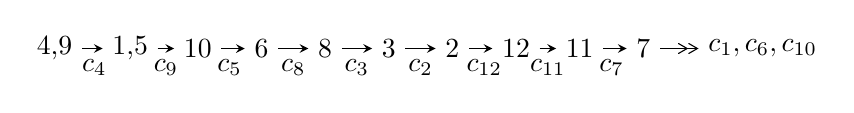
\begin{tikzpicture}[x=23pt, y=7pt]
	% node
	\node (A0) at (-1/8, 0) {4,9};
	\node (A1) at (17/16, 0) {1,5};
	\node (A2) at (17/8, 0) {10};
	\node (A3) at (25/8, 0) {6};
	\node (A4) at (33/8, 0) {8};
	\node (A5) at (41/8, 0) {3};
	\node (A6) at (49/8, 0) {2};
	\node (A7) at (57/8, 0) {12};
	\node (A8) at (65/8, 0) {11};
	\node (A9) at (73/8, 0) {7};
	\node (C1) at (1/2, -1) {$c_{4}$};
	\node (C2) at (13/8, -1) {$c_{9}$};
	\node (C3) at (21/8, -1) {$c_{5}$};
	\node (C4) at (29/8, -1) {$c_{8}$};
	\node (C5) at (37/8, -1) {$c_{3}$};
	\node (C6) at (45/8, -1) {$c_{2}$};
	\node (C7) at (53/8, -1) {$c_{12}$};
	\node (C8) at (61/8, -1) {$c_{11}$};
	\node (C9) at (69/8, -1) {$c_{7}$};
	\node (A10) at (11, 0) {$c_{1},c_{6},c_{10}$};

	% edge
	\draw[->,>=stealth]	
	(A0) edge (A1) (A1) edge (A2) (A2) edge (A3) (A3) edge (A4) (A4) edge (A5) (A5) edge (A6) (A6) edge (A7) (A7) edge (A8) (A8) edge (A9) ;
	\draw[->>,>={angle 60}]	
	(A9) edge (A10);
\end{tikzpicture} \\ 

\end{tabular} \\

\footnotetext{
The image of knot diagram is generated by the software ``\textbf{Draw programme}" developed by Andrew Bartholomew(\url{http://www.layer8.co.uk/maths/draw/index.htm\#Running-draw}), where we modified some parts for our purpose(\url{https://github.com/CATsTAILs/LinksPainter}).
}\phantom \\ \newline 
\centering \textbf{Ideals for irreducible components\footnotemark of $X_{\text{par}}$} 
 
\begin{align*}
I^u_{1}&=\langle 
-8.11138\times10^{47} u^{32}+5.57581\times10^{46} u^{31}+\cdots+2.13390\times10^{50} b+2.41977\times10^{50},\\
\phantom{I^u_{1}}&\phantom{= \langle  }-2.54097\times10^{51} u^{32}+4.05282\times10^{50} u^{31}+\cdots+3.69165\times10^{52} a+5.61038\times10^{53},\\
\phantom{I^u_{1}}&\phantom{= \langle  }u^{33}- u^{32}+\cdots-106 u+173\rangle \\
I^u_{2}&=\langle 
-3 u^{17}+4 u^{16}+\cdots+5 b+14,\;-19 u^{17}+2 u^{16}+\cdots+5 a+57,\;u^{18}-9 u^{16}+\cdots-2 u+1\rangle \\
\\
\end{align*}
\raggedright * 2 irreducible components of $\dim_{\mathbb{C}}=0$, with total 51 representations.\\
\footnotetext{All coefficients of polynomials are rational numbers. But the coefficients are sometimes approximated in decimal forms when there is not enough margin.}
\newpage
\renewcommand{\arraystretch}{1}
\centering \section*{I. $I^u_{1}= \langle -8.11\times10^{47} u^{32}+5.58\times10^{46} u^{31}+\cdots+2.13\times10^{50} b+2.42\times10^{50},\;-2.54\times10^{51} u^{32}+4.05\times10^{50} u^{31}+\cdots+3.69\times10^{52} a+5.61\times10^{53},\;u^{33}- u^{32}+\cdots-106 u+173 \rangle$}
\flushleft \textbf{(i) Arc colorings}\\
\begin{tabular}{m{7pt} m{180pt} m{7pt} m{180pt} }
\flushright $a_{4}=$&$\begin{pmatrix}1\\0\end{pmatrix}$ \\
\flushright $a_{9}=$&$\begin{pmatrix}0\\u\end{pmatrix}$ \\
\flushright $a_{1}=$&$\begin{pmatrix}0.0688301 u^{32}-0.0109783 u^{31}+\cdots-9.38616 u-15.1975\\0.00380120 u^{32}-0.000261296 u^{31}+\cdots-0.303063 u-1.13396\end{pmatrix}$ \\
\flushright $a_{5}=$&$\begin{pmatrix}1\\u^2\end{pmatrix}$ \\
\flushright $a_{10}=$&$\begin{pmatrix}0.0543141 u^{32}-0.00150099 u^{31}+\cdots-4.29999 u-10.4669\\0.0221013 u^{32}-0.00297101 u^{31}+\cdots-2.07083 u-4.65333\end{pmatrix}$ \\
\flushright $a_{6}=$&$\begin{pmatrix}0.0489761 u^{32}-0.00899494 u^{31}+\cdots-8.55348 u-10.6501\\0.0256145 u^{32}-0.00501638 u^{31}+\cdots-3.35159 u-6.23090\end{pmatrix}$ \\
\flushright $a_{8}=$&$\begin{pmatrix}u\\u\end{pmatrix}$ \\
\flushright $a_{3}=$&$\begin{pmatrix}- u^2+1\\- u^2\end{pmatrix}$ \\
\flushright $a_{2}=$&$\begin{pmatrix}0.0537482 u^{32}-0.00848860 u^{31}+\cdots-7.70974 u-11.3277\\0.0361202 u^{32}-0.00667465 u^{31}+\cdots-4.42265 u-7.79409\end{pmatrix}$ \\
\flushright $a_{12}=$&$\begin{pmatrix}0.112795 u^{32}-0.0212720 u^{31}+\cdots-14.8584 u-24.0719\\0.0284035 u^{32}-0.00624395 u^{31}+\cdots-4.33982 u-6.95902\end{pmatrix}$ \\
\flushright $a_{11}=$&$\begin{pmatrix}0.0229993 u^{32}+0.000676223 u^{31}+\cdots-2.29755 u-4.63975\\-0.00921351 u^{32}-0.000793791 u^{31}+\cdots-0.0683872 u+1.17380\end{pmatrix}$ \\
\flushright $a_{7}=$&$\begin{pmatrix}-0.0659945 u^{32}+0.0142976 u^{31}+\cdots+11.0084 u+15.2187\\-0.00761661 u^{32}-0.0000982334 u^{31}+\cdots+2.05310 u+2.41838\end{pmatrix}$\\&\end{tabular}
\flushleft \textbf{(ii) Obstruction class $= -1$}\\~\\
\flushleft \textbf{(iii) Cusp Shapes $= -0.280111 u^{32}+0.0673788 u^{31}+\cdots+28.5160 u+51.9527$}\\~\\
\newpage\renewcommand{\arraystretch}{1}
\flushleft \textbf{(iv) u-Polynomials at the component}\newline \\
\begin{tabular}{m{50pt}|m{274pt}}
Crossings & \hspace{64pt}u-Polynomials at each crossing \\
\hline $$\begin{aligned}c_{1}\end{aligned}$$&$\begin{aligned}
&u^{33}+31 u^{32}+\cdots-108 u-1
\end{aligned}$\\
\hline $$\begin{aligned}c_{2},c_{6}\end{aligned}$$&$\begin{aligned}
&u^{33}-3 u^{32}+\cdots+10 u+1
\end{aligned}$\\
\hline $$\begin{aligned}c_{3},c_{4},c_{8}\end{aligned}$$&$\begin{aligned}
&u^{33}- u^{32}+\cdots-106 u+173
\end{aligned}$\\
\hline $$\begin{aligned}c_{5}\end{aligned}$$&$\begin{aligned}
&u^{33}+u^{32}+\cdots+72271 u+18731
\end{aligned}$\\
\hline $$\begin{aligned}c_{7},c_{10}\end{aligned}$$&$\begin{aligned}
&u^{33}+u^{32}+\cdots+698 u+391
\end{aligned}$\\
\hline $$\begin{aligned}c_{9}\end{aligned}$$&$\begin{aligned}
&u^{33}-5 u^{32}+\cdots+28 u-11
\end{aligned}$\\
\hline $$\begin{aligned}c_{11}\end{aligned}$$&$\begin{aligned}
&u^{33}+55 u^{32}+\cdots-781200 u-152881
\end{aligned}$\\
\hline $$\begin{aligned}c_{12}\end{aligned}$$&$\begin{aligned}
&u^{33}- u^{32}+\cdots-428 u+187
\end{aligned}$\\
\hline
\end{tabular}\\~\\
\newpage\renewcommand{\arraystretch}{1}
\flushleft \textbf{(v) Riley Polynomials at the component}\newline \\
\begin{tabular}{m{50pt}|m{274pt}}
Crossings & \hspace{64pt}Riley Polynomials at each crossing \\
\hline $$\begin{aligned}c_{1}\end{aligned}$$&$\begin{aligned}
&y^{33}-45 y^{32}+\cdots-3432 y-1
\end{aligned}$\\
\hline $$\begin{aligned}c_{2},c_{6}\end{aligned}$$&$\begin{aligned}
&y^{33}+31 y^{32}+\cdots-108 y-1
\end{aligned}$\\
\hline $$\begin{aligned}c_{3},c_{4},c_{8}\end{aligned}$$&$\begin{aligned}
&y^{33}-43 y^{32}+\cdots+292880 y-29929
\end{aligned}$\\
\hline $$\begin{aligned}c_{5}\end{aligned}$$&$\begin{aligned}
&y^{33}+77 y^{32}+\cdots-6878739425 y-350850361
\end{aligned}$\\
\hline $$\begin{aligned}c_{7},c_{10}\end{aligned}$$&$\begin{aligned}
&y^{33}+55 y^{32}+\cdots-781200 y-152881
\end{aligned}$\\
\hline $$\begin{aligned}c_{9}\end{aligned}$$&$\begin{aligned}
&y^{33}-7 y^{32}+\cdots-778 y-121
\end{aligned}$\\
\hline $$\begin{aligned}c_{11}\end{aligned}$$&$\begin{aligned}
&y^{33}-149 y^{32}+\cdots-105634649180 y-23372600161
\end{aligned}$\\
\hline $$\begin{aligned}c_{12}\end{aligned}$$&$\begin{aligned}
&y^{33}+57 y^{32}+\cdots-214378 y-34969
\end{aligned}$\\
\hline
\end{tabular}\\~\\
\newpage\flushleft \textbf{(vi) Complex Volumes and Cusp Shapes}
$$\begin{array}{c|c|c}  
\text{Solutions to }I^u_{1}& \I (\text{vol} + \sqrt{-1}CS) & \text{Cusp shape}\\
 \hline 
\begin{aligned}
u &= \phantom{-}0.881268 + 0.494274 I \\
a &= \phantom{-}1.028140 - 0.103856 I \\
b &= \phantom{-}0.744044 - 0.822426 I\end{aligned}
 & -7.71312 - 1.78537 I & -0.85266 + 4.65753 I \\ \hline\begin{aligned}
u &= \phantom{-}0.881268 - 0.494274 I \\
a &= \phantom{-}1.028140 + 0.103856 I \\
b &= \phantom{-}0.744044 + 0.822426 I\end{aligned}
 & -7.71312 + 1.78537 I & -0.85266 - 4.65753 I \\ \hline\begin{aligned}
u &= \phantom{-}0.806093 + 0.733762 I \\
a &= -0.048706 + 0.852350 I \\
b &= -0.516099 + 0.675037 I\end{aligned}
 & -0.34629 + 2.42589 I & -3.38432 - 3.33398 I \\ \hline\begin{aligned}
u &= \phantom{-}0.806093 - 0.733762 I \\
a &= -0.048706 - 0.852350 I \\
b &= -0.516099 - 0.675037 I\end{aligned}
 & -0.34629 - 2.42589 I & -3.38432 + 3.33398 I \\ \hline\begin{aligned}
u &= -0.798281 + 0.311266 I \\
a &= -0.571033 - 0.836849 I \\
b &= -0.50701 + 2.28619 I\end{aligned}
 & -12.33120 + 1.02478 I & -6.59141 + 2.03554 I \\ \hline\begin{aligned}
u &= -0.798281 - 0.311266 I \\
a &= -0.571033 + 0.836849 I \\
b &= -0.50701 - 2.28619 I\end{aligned}
 & -12.33120 - 1.02478 I & -6.59141 - 2.03554 I \\ \hline\begin{aligned}
u &= \phantom{-}0.811379 + 0.055840 I \\
a &= -0.54698 + 1.54986 I \\
b &= -0.429316 + 0.085080 I\end{aligned}
 & -0.52878 + 4.48782 I & -5.13520 - 5.73220 I \\ \hline\begin{aligned}
u &= \phantom{-}0.811379 - 0.055840 I \\
a &= -0.54698 - 1.54986 I \\
b &= -0.429316 - 0.085080 I\end{aligned}
 & -0.52878 - 4.48782 I & -5.13520 + 5.73220 I \\ \hline\begin{aligned}
u &= -0.461701 + 0.612571 I \\
a &= \phantom{-}0.658166 - 0.583233 I \\
b &= -0.093739 + 0.146770 I\end{aligned}
 & \phantom{-}0.081645 + 1.028670 I & \phantom{-}0.74020 - 3.82977 I \\ \hline\begin{aligned}
u &= -0.461701 - 0.612571 I \\
a &= \phantom{-}0.658166 + 0.583233 I \\
b &= -0.093739 - 0.146770 I\end{aligned}
 & \phantom{-}0.081645 - 1.028670 I & \phantom{-}0.74020 + 3.82977 I\\
 \hline 
 \end{array}$$\newpage$$\begin{array}{c|c|c}  
\text{Solutions to }I^u_{1}& \I (\text{vol} + \sqrt{-1}CS) & \text{Cusp shape}\\
 \hline 
\begin{aligned}
u &= -0.520817 + 0.403957 I \\
a &= -0.656947 + 0.628673 I \\
b &= -0.343599 + 0.875931 I\end{aligned}
 & \phantom{-}0.07174 + 2.09017 I & -0.84653 - 3.88061 I \\ \hline\begin{aligned}
u &= -0.520817 - 0.403957 I \\
a &= -0.656947 - 0.628673 I \\
b &= -0.343599 - 0.875931 I\end{aligned}
 & \phantom{-}0.07174 - 2.09017 I & -0.84653 + 3.88061 I \\ \hline\begin{aligned}
u &= \phantom{-}0.541626 + 0.352089 I \\
a &= -1.57063 + 0.32219 I \\
b &= -0.995588 + 0.334486 I\end{aligned}
 & -3.54901 - 0.96370 I & -7.30947 + 1.19731 I \\ \hline\begin{aligned}
u &= \phantom{-}0.541626 - 0.352089 I \\
a &= -1.57063 - 0.32219 I \\
b &= -0.995588 - 0.334486 I\end{aligned}
 & -3.54901 + 0.96370 I & -7.30947 - 1.19731 I \\ \hline\begin{aligned}
u &= \phantom{-}1.367540 + 0.181430 I \\
a &= -0.883343 - 0.451036 I \\
b &= -1.89904 - 0.40011 I\end{aligned}
 & -5.14586 - 3.44515 I & -3.74377 + 8.43324 I \\ \hline\begin{aligned}
u &= \phantom{-}1.367540 - 0.181430 I \\
a &= -0.883343 + 0.451036 I \\
b &= -1.89904 + 0.40011 I\end{aligned}
 & -5.14586 + 3.44515 I & -3.74377 - 8.43324 I \\ \hline\begin{aligned}
u &= -0.263257 + 0.516809 I \\
a &= \phantom{-}0.905386 - 0.059376 I \\
b &= \phantom{-}0.061869 + 0.214108 I\end{aligned}
 & \phantom{-}0.112234 + 1.091570 I & \phantom{-}1.51179 - 6.02970 I \\ \hline\begin{aligned}
u &= -0.263257 - 0.516809 I \\
a &= \phantom{-}0.905386 + 0.059376 I \\
b &= \phantom{-}0.061869 - 0.214108 I\end{aligned}
 & \phantom{-}0.112234 - 1.091570 I & \phantom{-}1.51179 + 6.02970 I \\ \hline\begin{aligned}
u &= -1.46377\phantom{ +0.000000I} \\
a &= -0.611776\phantom{ +0.000000I} \\
b &= -1.74803\phantom{ +0.000000I}\end{aligned}
 & -3.79571\phantom{ +0.000000I} & -0.350320\phantom{ +0.000000I} \\ \hline\begin{aligned}
u &= -1.55168 + 0.23953 I \\
a &= \phantom{-}0.606082 - 0.442133 I \\
b &= \phantom{-}2.42916 + 0.21011 I\end{aligned}
 & -10.65780 + 3.51663 I & -5.96026 + 0. I\phantom{ +0.000000I}\\
 \hline 
 \end{array}$$\newpage$$\begin{array}{c|c|c}  
\text{Solutions to }I^u_{1}& \I (\text{vol} + \sqrt{-1}CS) & \text{Cusp shape}\\
 \hline 
\begin{aligned}
u &= -1.55168 - 0.23953 I \\
a &= \phantom{-}0.606082 + 0.442133 I \\
b &= \phantom{-}2.42916 - 0.21011 I\end{aligned}
 & -10.65780 - 3.51663 I & -5.96026 + 0. I\phantom{ +0.000000I} \\ \hline\begin{aligned}
u &= \phantom{-}1.56741 + 0.23862 I \\
a &= \phantom{-}0.584803 - 0.034792 I \\
b &= \phantom{-}1.91823 + 0.02308 I\end{aligned}
 & -7.35813 - 4.59771 I & \phantom{-0.000000 } 0 \\ \hline\begin{aligned}
u &= \phantom{-}1.56741 - 0.23862 I \\
a &= \phantom{-}0.584803 + 0.034792 I \\
b &= \phantom{-}1.91823 - 0.02308 I\end{aligned}
 & -7.35813 + 4.59771 I & \phantom{-0.000000 } 0 \\ \hline\begin{aligned}
u &= -0.95012 + 1.51122 I \\
a &= -0.549793 - 0.409182 I \\
b &= -0.633085 + 0.187322 I\end{aligned}
 & -14.0224 + 4.9505 I & \phantom{-0.000000 } 0 \\ \hline\begin{aligned}
u &= -0.95012 - 1.51122 I \\
a &= -0.549793 + 0.409182 I \\
b &= -0.633085 - 0.187322 I\end{aligned}
 & -14.0224 - 4.9505 I & \phantom{-0.000000 } 0 \\ \hline\begin{aligned}
u &= \phantom{-}1.79395 + 0.15288 I \\
a &= \phantom{-}0.565816 - 0.803329 I \\
b &= \phantom{-}1.74296 - 0.32540 I\end{aligned}
 & \phantom{-}17.5407 - 3.2542 I & \phantom{-0.000000 } 0 \\ \hline\begin{aligned}
u &= \phantom{-}1.79395 - 0.15288 I \\
a &= \phantom{-}0.565816 + 0.803329 I \\
b &= \phantom{-}1.74296 + 0.32540 I\end{aligned}
 & \phantom{-}17.5407 + 3.2542 I & \phantom{-0.000000 } 0 \\ \hline\begin{aligned}
u &= -1.79808 + 0.17463 I \\
a &= -0.774547 + 0.627665 I \\
b &= -2.05265 + 0.43342 I\end{aligned}
 & -17.5402 + 4.7342 I & \phantom{-0.000000 } 0 \\ \hline\begin{aligned}
u &= -1.79808 - 0.17463 I \\
a &= -0.774547 - 0.627665 I \\
b &= -2.05265 - 0.43342 I\end{aligned}
 & -17.5402 - 4.7342 I & \phantom{-0.000000 } 0 \\ \hline\begin{aligned}
u &= \phantom{-}1.81040 + 0.47252 I \\
a &= \phantom{-}0.816894 + 0.399455 I \\
b &= \phantom{-}2.24901 + 0.45557 I\end{aligned}
 & \phantom{-}16.7809 - 12.3351 I & \phantom{-0.000000 } 0\\
 \hline 
 \end{array}$$\newpage$$\begin{array}{c|c|c}  
\text{Solutions to }I^u_{1}& \I (\text{vol} + \sqrt{-1}CS) & \text{Cusp shape}\\
 \hline 
\begin{aligned}
u &= \phantom{-}1.81040 - 0.47252 I \\
a &= \phantom{-}0.816894 - 0.399455 I \\
b &= \phantom{-}2.24901 - 0.45557 I\end{aligned}
 & \phantom{-}16.7809 + 12.3351 I & \phantom{-0.000000 } 0 \\ \hline\begin{aligned}
u &= -2.00385 + 0.04235 I \\
a &= \phantom{-}0.612520 - 0.356931 I \\
b &= \phantom{-}1.69886 - 0.37474 I\end{aligned}
 & -11.89190 + 2.84171 I & \phantom{-0.000000 } 0 \\ \hline\begin{aligned}
u &= -2.00385 - 0.04235 I \\
a &= \phantom{-}0.612520 + 0.356931 I \\
b &= \phantom{-}1.69886 + 0.37474 I\end{aligned}
 & -11.89190 - 2.84171 I & \phantom{-0.000000 } 0\\
 \hline 
 \end{array}$$\newpage\newpage\renewcommand{\arraystretch}{1}
\centering \section*{II. $I^u_{2}= \langle -3 u^{17}+4 u^{16}+\cdots+5 b+14,\;-19 u^{17}+2 u^{16}+\cdots+5 a+57,\;u^{18}-9 u^{16}+\cdots-2 u+1 \rangle$}
\flushleft \textbf{(i) Arc colorings}\\
\begin{tabular}{m{7pt} m{180pt} m{7pt} m{180pt} }
\flushright $a_{4}=$&$\begin{pmatrix}1\\0\end{pmatrix}$ \\
\flushright $a_{9}=$&$\begin{pmatrix}0\\u\end{pmatrix}$ \\
\flushright $a_{1}=$&$\begin{pmatrix}\frac{19}{5} u^{17}-\frac{2}{5} u^{16}+\cdots-\frac{62}{5} u-\frac{57}{5}\\\frac{3}{5} u^{17}-\frac{4}{5} u^{16}+\cdots-\frac{9}{5} u-\frac{14}{5}\end{pmatrix}$ \\
\flushright $a_{5}=$&$\begin{pmatrix}1\\u^2\end{pmatrix}$ \\
\flushright $a_{10}=$&$\begin{pmatrix}\frac{9}{5} u^{17}-\frac{2}{5} u^{16}+\cdots-\frac{12}{5} u-\frac{47}{5}\\-\frac{9}{5} u^{17}-\frac{18}{5} u^{16}+\cdots-\frac{8}{5} u+\frac{2}{5}\end{pmatrix}$ \\
\flushright $a_{6}=$&$\begin{pmatrix}-5.40000 u^{17}-3.80000 u^{16}+\cdots+4.20000 u+11.2000\\-2.60000 u^{17}-3.20000 u^{16}+\cdots-2.20000 u+3.80000\end{pmatrix}$ \\
\flushright $a_{8}=$&$\begin{pmatrix}u\\u\end{pmatrix}$ \\
\flushright $a_{3}=$&$\begin{pmatrix}- u^2+1\\- u^2\end{pmatrix}$ \\
\flushright $a_{2}=$&$\begin{pmatrix}2 u^{17}-3 u^{16}+\cdots-13 u-6\\-\frac{4}{5} u^{17}-\frac{28}{5} u^{16}+\cdots-\frac{33}{5} u-\frac{3}{5}\end{pmatrix}$ \\
\flushright $a_{12}=$&$\begin{pmatrix}\frac{12}{5} u^{17}-\frac{16}{5} u^{16}+\cdots-\frac{76}{5} u-\frac{41}{5}\\- u^{17}-5 u^{16}+\cdots-6 u^2-6 u\end{pmatrix}$ \\
\flushright $a_{11}=$&$\begin{pmatrix}\frac{2}{5} u^{17}-\frac{16}{5} u^{16}+\cdots-\frac{26}{5} u-\frac{31}{5}\\-3.20000 u^{17}-6.40000 u^{16}+\cdots-4.40000 u+3.60000\end{pmatrix}$ \\
\flushright $a_{7}=$&$\begin{pmatrix}-6.60000 u^{17}-6.20000 u^{16}+\cdots+7.80000 u+15.8000\\-3.40000 u^{17}-5.80000 u^{16}+\cdots-3.80000 u+7.20000\end{pmatrix}$\\&\end{tabular}
\flushleft \textbf{(ii) Obstruction class $= 1$}\\~\\
\flushleft \textbf{(iii) Cusp Shapes $= -2 u^{17}+5 u^{16}+27 u^{15}-34 u^{14}-125 u^{13}+95 u^{12}+270 u^{11}-122 u^{10}-239 u^9+41 u^8-99 u^7+37 u^6+384 u^5+32 u^4-257 u^3-88 u^2+25 u+15$}\\~\\
\newpage\renewcommand{\arraystretch}{1}
\flushleft \textbf{(iv) u-Polynomials at the component}\newline \\
\begin{tabular}{m{50pt}|m{274pt}}
Crossings & \hspace{64pt}u-Polynomials at each crossing \\
\hline $$\begin{aligned}c_{1}\end{aligned}$$&$\begin{aligned}
&u^{18}-12 u^{17}+\cdots-16 u+1
\end{aligned}$\\
\hline $$\begin{aligned}c_{2}\end{aligned}$$&$\begin{aligned}
&u^{18}-2 u^{17}+\cdots-2 u+1
\end{aligned}$\\
\hline $$\begin{aligned}c_{3},c_{4}\end{aligned}$$&$\begin{aligned}
&u^{18}-9 u^{16}+\cdots-2 u+1
\end{aligned}$\\
\hline $$\begin{aligned}c_{5}\end{aligned}$$&$\begin{aligned}
&u^{18}+7 u^{16}+\cdots+u+1
\end{aligned}$\\
\hline $$\begin{aligned}c_{6}\end{aligned}$$&$\begin{aligned}
&u^{18}+2 u^{17}+\cdots+2 u+1
\end{aligned}$\\
\hline $$\begin{aligned}c_{7}\end{aligned}$$&$\begin{aligned}
&u^{18}+8 u^{16}+\cdots+4 u^2+1
\end{aligned}$\\
\hline $$\begin{aligned}c_{8}\end{aligned}$$&$\begin{aligned}
&u^{18}-9 u^{16}+\cdots+2 u+1
\end{aligned}$\\
\hline $$\begin{aligned}c_{9}\end{aligned}$$&$\begin{aligned}
&u^{18}-6 u^{17}+\cdots-2 u+1
\end{aligned}$\\
\hline $$\begin{aligned}c_{10}\end{aligned}$$&$\begin{aligned}
&u^{18}+8 u^{16}+\cdots+4 u^2+1
\end{aligned}$\\
\hline $$\begin{aligned}c_{11}\end{aligned}$$&$\begin{aligned}
&u^{18}+16 u^{17}+\cdots+8 u+1
\end{aligned}$\\
\hline $$\begin{aligned}c_{12}\end{aligned}$$&$\begin{aligned}
&u^{18}+11 u^{16}+\cdots-2 u+1
\end{aligned}$\\
\hline
\end{tabular}\\~\\
\newpage\renewcommand{\arraystretch}{1}
\flushleft \textbf{(v) Riley Polynomials at the component}\newline \\
\begin{tabular}{m{50pt}|m{274pt}}
Crossings & \hspace{64pt}Riley Polynomials at each crossing \\
\hline $$\begin{aligned}c_{1}\end{aligned}$$&$\begin{aligned}
&y^{18}-20 y^{16}+\cdots-24 y+1
\end{aligned}$\\
\hline $$\begin{aligned}c_{2},c_{6}\end{aligned}$$&$\begin{aligned}
&y^{18}+12 y^{17}+\cdots+16 y+1
\end{aligned}$\\
\hline $$\begin{aligned}c_{3},c_{4},c_{8}\end{aligned}$$&$\begin{aligned}
&y^{18}-18 y^{17}+\cdots-20 y+1
\end{aligned}$\\
\hline $$\begin{aligned}c_{5}\end{aligned}$$&$\begin{aligned}
&y^{18}+14 y^{17}+\cdots-3 y+1
\end{aligned}$\\
\hline $$\begin{aligned}c_{7},c_{10}\end{aligned}$$&$\begin{aligned}
&y^{18}+16 y^{17}+\cdots+8 y+1
\end{aligned}$\\
\hline $$\begin{aligned}c_{9}\end{aligned}$$&$\begin{aligned}
&y^{18}+2 y^{17}+\cdots-10 y+1
\end{aligned}$\\
\hline $$\begin{aligned}c_{11}\end{aligned}$$&$\begin{aligned}
&y^{18}-24 y^{17}+\cdots+4 y+1
\end{aligned}$\\
\hline $$\begin{aligned}c_{12}\end{aligned}$$&$\begin{aligned}
&y^{18}+22 y^{17}+\cdots+14 y+1
\end{aligned}$\\
\hline
\end{tabular}\\~\\
\newpage\flushleft \textbf{(vi) Complex Volumes and Cusp Shapes}
$$\begin{array}{c|c|c}  
\text{Solutions to }I^u_{2}& \I (\text{vol} + \sqrt{-1}CS) & \text{Cusp shape}\\
 \hline 
\begin{aligned}
u &= \phantom{-}0.085759 + 1.011970 I \\
a &= \phantom{-}0.071482 + 0.659946 I \\
b &= -0.330517 + 0.071724 I\end{aligned}
 & -1.08613 - 0.96816 I & -6.34211 + 0.57071 I \\ \hline\begin{aligned}
u &= \phantom{-}0.085759 - 1.011970 I \\
a &= \phantom{-}0.071482 - 0.659946 I \\
b &= -0.330517 - 0.071724 I\end{aligned}
 & -1.08613 + 0.96816 I & -6.34211 - 0.57071 I \\ \hline\begin{aligned}
u &= -1.114560 + 0.293820 I \\
a &= -0.931989 + 0.046707 I \\
b &= -1.33734 - 0.90053 I\end{aligned}
 & -8.46698 + 1.31286 I & -9.83068 + 0.32018 I \\ \hline\begin{aligned}
u &= -1.114560 - 0.293820 I \\
a &= -0.931989 - 0.046707 I \\
b &= -1.33734 + 0.90053 I\end{aligned}
 & -8.46698 - 1.31286 I & -9.83068 - 0.32018 I \\ \hline\begin{aligned}
u &= \phantom{-}1.300570 + 0.029273 I \\
a &= -0.536713 - 1.019510 I \\
b &= -1.28702 - 0.60196 I\end{aligned}
 & -2.94807 - 4.42128 I & -4.69559 + 5.41775 I \\ \hline\begin{aligned}
u &= \phantom{-}1.300570 - 0.029273 I \\
a &= -0.536713 + 1.019510 I \\
b &= -1.28702 + 0.60196 I\end{aligned}
 & -2.94807 + 4.42128 I & -4.69559 - 5.41775 I \\ \hline\begin{aligned}
u &= -1.306820 + 0.073942 I \\
a &= \phantom{-}0.030062 + 0.945777 I \\
b &= \phantom{-}0.663121 + 0.218291 I\end{aligned}
 & -3.48940 + 1.60644 I & -4.34335 - 1.67805 I \\ \hline\begin{aligned}
u &= -1.306820 - 0.073942 I \\
a &= \phantom{-}0.030062 - 0.945777 I \\
b &= \phantom{-}0.663121 - 0.218291 I\end{aligned}
 & -3.48940 - 1.60644 I & -4.34335 + 1.67805 I \\ \hline\begin{aligned}
u &= \phantom{-}1.232400 + 0.491104 I \\
a &= \phantom{-}0.340655 - 0.011913 I \\
b &= \phantom{-}1.05787 - 1.88552 I\end{aligned}
 & -12.53040 - 2.23082 I & -8.19150 + 3.26212 I \\ \hline\begin{aligned}
u &= \phantom{-}1.232400 - 0.491104 I \\
a &= \phantom{-}0.340655 + 0.011913 I \\
b &= \phantom{-}1.05787 + 1.88552 I\end{aligned}
 & -12.53040 + 2.23082 I & -8.19150 - 3.26212 I\\
 \hline 
 \end{array}$$\newpage$$\begin{array}{c|c|c}  
\text{Solutions to }I^u_{2}& \I (\text{vol} + \sqrt{-1}CS) & \text{Cusp shape}\\
 \hline 
\begin{aligned}
u &= \phantom{-}1.329640 + 0.238506 I \\
a &= -1.026160 - 0.341518 I \\
b &= -2.02234 - 0.39359 I\end{aligned}
 & -5.47647 - 2.87572 I & -10.17496 - 1.27830 I \\ \hline\begin{aligned}
u &= \phantom{-}1.329640 - 0.238506 I \\
a &= -1.026160 + 0.341518 I \\
b &= -2.02234 + 0.39359 I\end{aligned}
 & -5.47647 + 2.87572 I & -10.17496 + 1.27830 I \\ \hline\begin{aligned}
u &= -0.375312 + 0.293384 I \\
a &= \phantom{-}1.52275 - 1.15299 I \\
b &= -0.663240 - 0.618071 I\end{aligned}
 & -0.093430 - 0.496699 I & -2.79813 + 0.04829 I \\ \hline\begin{aligned}
u &= -0.375312 - 0.293384 I \\
a &= \phantom{-}1.52275 + 1.15299 I \\
b &= -0.663240 + 0.618071 I\end{aligned}
 & -0.093430 + 0.496699 I & -2.79813 - 0.04829 I \\ \hline\begin{aligned}
u &= -1.52906 + 0.23255 I \\
a &= \phantom{-}0.647405 - 0.190244 I \\
b &= \phantom{-}2.05285 - 0.17653 I\end{aligned}
 & -7.41546 + 5.53534 I & -5.08064 - 8.15204 I \\ \hline\begin{aligned}
u &= -1.52906 - 0.23255 I \\
a &= \phantom{-}0.647405 + 0.190244 I \\
b &= \phantom{-}2.05285 + 0.17653 I\end{aligned}
 & -7.41546 - 5.53534 I & -5.08064 + 8.15204 I \\ \hline\begin{aligned}
u &= \phantom{-}0.377398 + 0.043983 I \\
a &= -1.11749 + 2.90937 I \\
b &= -0.133373 + 0.724783 I\end{aligned}
 & \phantom{-}0.38303 + 4.11760 I & \phantom{-}1.95695 - 4.69583 I \\ \hline\begin{aligned}
u &= \phantom{-}0.377398 - 0.043983 I \\
a &= -1.11749 - 2.90937 I \\
b &= -0.133373 - 0.724783 I\end{aligned}
 & \phantom{-}0.38303 - 4.11760 I & \phantom{-}1.95695 + 4.69583 I\\
 \hline 
 \end{array}$$\newpage
\newpage\renewcommand{\arraystretch}{1}
\centering \section*{ III. u-Polynomials}
\begin{tabular}{m{50pt}|m{274pt}}
Crossings & \hspace{64pt}u-Polynomials at each crossing \\
\hline $$\begin{aligned}c_{1}\end{aligned}$$&$\begin{aligned}
&(u^{18}-12 u^{17}+\cdots-16 u+1)(u^{33}+31 u^{32}+\cdots-108 u-1)
\end{aligned}$\\
\hline $$\begin{aligned}c_{2}\end{aligned}$$&$\begin{aligned}
&(u^{18}-2 u^{17}+\cdots-2 u+1)(u^{33}-3 u^{32}+\cdots+10 u+1)
\end{aligned}$\\
\hline $$\begin{aligned}c_{3},c_{4}\end{aligned}$$&$\begin{aligned}
&(u^{18}-9 u^{16}+\cdots-2 u+1)(u^{33}- u^{32}+\cdots-106 u+173)
\end{aligned}$\\
\hline $$\begin{aligned}c_{5}\end{aligned}$$&$\begin{aligned}
&(u^{18}+7 u^{16}+\cdots+u+1)(u^{33}+u^{32}+\cdots+72271 u+18731)
\end{aligned}$\\
\hline $$\begin{aligned}c_{6}\end{aligned}$$&$\begin{aligned}
&(u^{18}+2 u^{17}+\cdots+2 u+1)(u^{33}-3 u^{32}+\cdots+10 u+1)
\end{aligned}$\\
\hline $$\begin{aligned}c_{7}\end{aligned}$$&$\begin{aligned}
&(u^{18}+8 u^{16}+\cdots+4 u^2+1)(u^{33}+u^{32}+\cdots+698 u+391)
\end{aligned}$\\
\hline $$\begin{aligned}c_{8}\end{aligned}$$&$\begin{aligned}
&(u^{18}-9 u^{16}+\cdots+2 u+1)(u^{33}- u^{32}+\cdots-106 u+173)
\end{aligned}$\\
\hline $$\begin{aligned}c_{9}\end{aligned}$$&$\begin{aligned}
&(u^{18}-6 u^{17}+\cdots-2 u+1)(u^{33}-5 u^{32}+\cdots+28 u-11)
\end{aligned}$\\
\hline $$\begin{aligned}c_{10}\end{aligned}$$&$\begin{aligned}
&(u^{18}+8 u^{16}+\cdots+4 u^2+1)(u^{33}+u^{32}+\cdots+698 u+391)
\end{aligned}$\\
\hline $$\begin{aligned}c_{11}\end{aligned}$$&$\begin{aligned}
&(u^{18}+16 u^{17}+\cdots+8 u+1)(u^{33}+55 u^{32}+\cdots-781200 u-152881)
\end{aligned}$\\
\hline $$\begin{aligned}c_{12}\end{aligned}$$&$\begin{aligned}
&(u^{18}+11 u^{16}+\cdots-2 u+1)(u^{33}- u^{32}+\cdots-428 u+187)
\end{aligned}$\\
\hline
\end{tabular}\newpage\renewcommand{\arraystretch}{1}
\centering \section*{ IV. Riley Polynomials}
\begin{tabular}{m{50pt}|m{274pt}}
Crossings & \hspace{64pt}Riley Polynomials at each crossing \\
\hline $$\begin{aligned}c_{1}\end{aligned}$$&$\begin{aligned}
&(y^{18}-20 y^{16}+\cdots-24 y+1)(y^{33}-45 y^{32}+\cdots-3432 y-1)
\end{aligned}$\\
\hline $$\begin{aligned}c_{2},c_{6}\end{aligned}$$&$\begin{aligned}
&(y^{18}+12 y^{17}+\cdots+16 y+1)(y^{33}+31 y^{32}+\cdots-108 y-1)
\end{aligned}$\\
\hline $$\begin{aligned}c_{3},c_{4},c_{8}\end{aligned}$$&$\begin{aligned}
&(y^{18}-18 y^{17}+\cdots-20 y+1)(y^{33}-43 y^{32}+\cdots+292880 y-29929)
\end{aligned}$\\
\hline $$\begin{aligned}c_{5}\end{aligned}$$&$\begin{aligned}
&(y^{18}+14 y^{17}+\cdots-3 y+1)\\
&\cdot(y^{33}+77 y^{32}+\cdots-6878739425 y-350850361)
\end{aligned}$\\
\hline $$\begin{aligned}c_{7},c_{10}\end{aligned}$$&$\begin{aligned}
&(y^{18}+16 y^{17}+\cdots+8 y+1)(y^{33}+55 y^{32}+\cdots-781200 y-152881)
\end{aligned}$\\
\hline $$\begin{aligned}c_{9}\end{aligned}$$&$\begin{aligned}
&(y^{18}+2 y^{17}+\cdots-10 y+1)(y^{33}-7 y^{32}+\cdots-778 y-121)
\end{aligned}$\\
\hline $$\begin{aligned}c_{11}\end{aligned}$$&$\begin{aligned}
&(y^{18}-24 y^{17}+\cdots+4 y+1)\\
&\cdot(y^{33}-149 y^{32}+\cdots-105634649180 y-23372600161)
\end{aligned}$\\
\hline $$\begin{aligned}c_{12}\end{aligned}$$&$\begin{aligned}
&(y^{18}+22 y^{17}+\cdots+14 y+1)(y^{33}+57 y^{32}+\cdots-214378 y-34969)
\end{aligned}$\\
\hline
\end{tabular}
\vskip 2pc
\end{document}